\documentclass[11pt]{article}

\usepackage[margin=1in]{geometry}
\usepackage{amsmath,amssymb,booktabs,longtable,array}
\usepackage{graphicx}
\usepackage{hyperref}
\usepackage{natbib}
\usepackage{enumitem}
\usepackage{microtype}

\title{RAPM DECOMP: An Additive Decomposition of Regularized Adjusted Plus-Minus}
\author{Russell Thomas}
\date{Draft of June 2026}

\begin{document}
\maketitle

\begin{abstract}
Regularized adjusted plus-minus is useful because it estimates player impact
while controlling for the other nine players on the floor.  It is also hard to
explain because the usual public object is a single coefficient.  This paper
introduces RAPM DECOMP, an additive possession-value framework that decomposes
offensive and defensive RAPM into first-chance value and second-chance value
while preserving the lineup-adjusted design that makes RAPM useful.

The central public identity is first-chance RAPM:
\[
\text{oFC} = \text{oEFG} + \text{oFT} + \text{oTOV}.
\]
Here \texttt{oEFG} is adjusted first-chance field-goal value, \texttt{oFT} is
adjusted first-chance free-throw value, and \texttt{oTOV} is point-valued
first-chance turnover value.  The scoring branch \texttt{oEFG + oFT} is
\texttt{oTS}, an adjusted first-chance points-per-shot RAPM term.  Total
offense then adds post-miss extension value:
\[
\text{off} = \text{oFC} + \text{oSC}.
\]
The same accounting holds on defense with \texttt{dFC}, \texttt{dTS}, and
\texttt{dSC}, after sign-flipping defensive factors so positive values are good
for the player's team.

On the current 2024--2026 NBA public export, 797 player rows and 7.73 million
possession-weighted player observations have maximum rounded residual 0.001
points per 100 possessions between actual RAPM and the factor sum, with
possession-weighted mean absolute residual 0.000255.  The long 1997--2026
export contains 2,859 player rows and 71.03 million possession-weighted
observations with the same maximum rounded residual.  The claim is not that
RAPM DECOMP solves basketball causality.  The claim is narrower and auditable:
when adjusted value is published, its books can be kept.  Actual RAPM can be
shown beside first-chance scoring value, first-chance turnover value, and
second-chance value, with almost zero public accounting error.
\end{abstract}

\clearpage

\section{Introduction}

Basketball statistics are often split into two unsatisfying families.  Box-score
and tracking-based statistics can explain what happened in basketball terms,
but they can miss effects that appear only through teammates, opponents,
spacing, screening, rotations, and lineup context.  Adjusted plus-minus models
control for teammates and opponents, but they usually return a single number.
That number can be valuable, but it is quiet.  A player can have a large RAPM
coefficient because his lineups generate better first shots, draw more valuable
free throws, avoid first-chance turnovers, extend possessions after misses,
suppress opponent shot value, or combine several smaller effects.  The
coefficient itself does not say which channels carried the value.

RAPM DECOMP keeps the adjusted-lineup discipline of RAPM and opens the
coefficient into basketball accounting terms.  It does not regress a player
rating on box-score summaries.  It stays at the possession level, where RAPM is
estimated.  Each component is a mechanically defined target attached to the same
lineup rows.  The model asks: if the dependent variable is first-chance shot
value instead of total point differential, which players are associated with
that value after controlling for teammates and opponents?  The same question is
asked for free throws, turnovers, and second chances.

The key constraint is additivity.  Public decomposition columns should not be
labels placed beside a total coefficient.  They should be in common units, with
an explicit test against the parent coefficient.  RAPM DECOMP does this in
points per 100 possessions.  On offense, the first-chance structure is:
\[
\text{oFC}
= \text{oEFG}
+ \text{oFT}
+ \text{oTOV}.
\]
Here \texttt{oFC} is offensive first-chance RAPM: effective-field-goal value,
free-throw value, and turnover value before the first offensive rebound.  The
scoring branch is:
\[
\text{oTS} = \text{oEFG} + \text{oFT},
\]
where \texttt{oTS} is adjusted first-chance points-per-shot value.  Total
offense is:
\[
\text{off} = \text{oFC} + \text{oSC}.
\]
\texttt{oSC} is offensive second-chance value, the post-miss value generated
after the first offensive rebound opportunity.  The same structure holds on
defense:
\[
\text{dFC} = \text{dEFG} + \text{dFT} + \text{dTOV}, \qquad
\text{dTS} = \text{dEFG} + \text{dFT}, \qquad
\text{def} = \text{dFC} + \text{dSC}.
\]
Defensive factors are sign-flipped so that positive means good for the
player's team.  The residual is not a fifth basketball term.  It is the
measured difference between actual RAPM and the published factor sum.

This paper makes three contributions.  First, it defines an additive
RAPM-decomposition operator: component targets are solved with the same
lineup-adjusted ridge machinery as total RAPM.  Second, it gives a basketball
schema for the largest scoring channels: first-chance true-shooting value,
first-chance turnover value, and second-chance value, with true-shooting value
opened into EFG and free-throw value.  Third, it reports the public residual
between actual RAPM and the factor sum in current exports and shows player
profiles that are recognizable as basketball rather than arbitrary
post-processing.

\section{Background and Motivation}

Adjusted plus-minus treats a stint or possession as an observation and the
players on the floor as signed predictors.  Ridge regularization stabilizes the
estimate in the presence of repeated lineups, collinearity, and low-minute
players.  The resulting RAPM coefficient is a partial association between a
player and team scoring margin, conditional on the other players in the row.
This conditional structure is the core reason RAPM matters.

RAPM also has well-known limits.  Players are not randomly assigned to lineups.
Roles, coaches, teammates, opponents, score effects, and era effects all matter.
Regularization reduces variance, but it does not create a randomized
experiment.  RAPM should therefore be read as adjusted evidence, not as a pure
causal treatment effect.

The usual public workaround is to blend adjusted plus-minus with box-score,
tracking, or scouting priors.  Those hybrids can be excellent rating systems,
but they answer a different question from decomposition.  A prior-centered
metric asks how to stabilize a player rating.  RAPM DECOMP asks where the
adjusted rating lands in the possession economy.  Priors can later be attached
to each channel, but the channel itself should have a mechanical target.

The method also differs from a box-score explanation layer.  A player-level
summary such as rim attempts, assists, turnover percentage, or offensive
rebound rate can help explain a component, but it is not the component.  The
component is estimated from lineup-adjusted possession outcomes.  For example,
offensive rim-frequency value is not simply the player's own rim-attempt rate.
It is the adjusted value of lineups shifting first-chance shot value toward or
away from the rim while that player is on offense.

The public lineage begins with adjusted plus-minus: estimate player effects
from scoring margin while controlling for all players on the floor.  Rosenbaum's
early public work introduced the broad idea to basketball audiences, and Sill's
regularized formulation made the approach more practical by using shrinkage and
out-of-sample testing.  Later possession-value models, including work by
Cervone, D'Amour, Bornn, and Goldsberry, showed that basketball possessions can
be valued as evolving states rather than only as final outcomes.

RAPM DECOMP sits between those traditions.  Like RAPM, it uses lineup-adjusted
estimation rather than assigning credit directly from the event log.  Like
possession-value work, it insists that the scoreboard can be opened into
smaller states and events.  The distinct move is to keep the RAPM design matrix
and change the target.  The model does not ask which player recorded a
box-score event.  It asks which players are associated with possession-value
channels after the same teammate and opponent controls used in RAPM.

\section{RAPM as an Operator}

Let $j$ index possession rows.  Let $y_j$ be a target, such as total point
differential, first-chance EFG value, free-throw value, turnover value, or
second-chance value.  Let $w_j$ be an observation weight.  Let $X$ be the sparse
player design matrix.  In a simplified single-block notation, $X_{jp}=+1$ when
player $p$ is on the offensive side of row $j$, $X_{jp}=-1$ when player $p$ is
on the defensive side, and $X_{jp}=0$ otherwise.  Production solves use
separate offensive and defensive columns and can apply different penalties by
side, but the notation is enough to state the idea.  The ridge estimate is
\[
\hat{\beta}_y =
\arg\min_{\beta}
\sum_j w_j (y_j - X_j\beta)^2 + \lambda \|\beta\|_2^2 .
\]
Define $R(y)=\hat{\beta}_y$, the regularized lineup-adjustment operator applied
to target $y$.

If a row target decomposes as $y=a+b+c$, it is tempting to assume
$R(y)=R(a)+R(b)+R(c)$.  RAPM DECOMP does not rely on that assumption.  Separate
ridge solves, centering, nuisance terms, and rounded CSV exports can perturb raw
coefficient sums even when row algebra is exact.  The public decomposition
therefore measures the residual directly:
\[
\text{Residual} = R(y) - \sum_k R(c_k),
\]
where $R(y)$ is the actual parent RAPM coefficient and $R(c_k)$ are the
published factor coefficients.

This ordering matters.  A component coefficient is meaningful only if the
target it came from is meaningful.  If the row construction is wrong, a tidy
player table is not evidence.  If the row construction is sound but the factors
do not add back to the actual parent coefficient, the difference is the public
decomposition error.  The empirical claim here is that this error is
rounding-scale in the finished exports.

\section{The Decomposition Tree}

The public RAPM DECOMP table uses a nested decomposition.  At the highest level:
\[
\text{Net RAPM} = \text{Offense} + \text{Defense}.
\]
Within offense:
\[
\text{Offense} = \text{oFC} + \text{oSC},
\]
and within defense:
\[
\text{Defense} = \text{dFC} + \text{dSC}.
\]
First-chance value is the value before the first offensive rebound opportunity.
Second-chance value is the value after the first offensive miss has created an
extension opportunity.  This separation keeps offensive rebounding and the
points that follow an extended possession from being hidden inside first-shot
quality.

Within first chance:
\[
\text{oFC} = \text{oTS} + \text{oTOV},
\qquad
\text{dFC} = \text{dTS} + \text{dTOV}.
\]
\texttt{oTOV} is not a turnover-rate coefficient.  It is point-valued lost
first-chance opportunity.  A true first-chance turnover is a possession-ending
turnover before a first-chance shot or completed free-throw sequence.  If a
possession already produced a make, field-goal attempt, or completed
free-throw sequence, a later terminal turnover does not retroactively erase
that first-chance scoring.  This guard is small in code and large in meaning:
the same possession should not be counted both as realized first-chance scoring
and as lost first-chance scoring value.

Within first-chance scoring:
\[
\text{oTS} = \text{oEFG} + \text{oFT},
\qquad
\text{dTS} = \text{dEFG} + \text{dFT}.
\]
The term \texttt{oTS} should be read as adjusted first-chance points-per-shot
value, not as a box-score true-shooting percentage.  It combines field-goal
shot value and free-throw value on the same point scale.  The field-goal branch
can be opened further:
\[
\text{EFG Value}
= \text{EFG Baseline}
+ \text{Rim Frequency} + \text{Rim Conversion}
+ \text{Midrange Frequency} + \text{Midrange Conversion}
+ \text{Three-Point Frequency} + \text{Three-Point Conversion}.
\]
The baseline term keeps the unatomized part of first-chance field-goal value
inside the EFG branch, so it is not misassigned to free throws, turnovers,
second chance, or residual.

Free-throw value can also be opened:
\[
\text{Free-Throw Value}
= \text{Trip Frequency Value} + \text{Trip Severity Value}.
\]
Frequency credits the creation of first-chance free-throw trips at the average
trip value in the loaded sample.  Severity is the value above or below that
average trip, combining trip type and free-throw shooting.  The current split
is intentionally conservative: it separates creating trips from the value of
those trips, but it does not yet separate trip type from shooter conversion in
the public table.

\section{Public Units and Run Specification}

Production RAPM runs can include score-margin by period terms, season-phase
fixed effects, time decay, age terms, or other nuisance blocks.  These terms are
not basketball skill components.  They are included to keep player coefficients
from absorbing broad context shifts.  A public row must therefore be read with
its run specification.  The primary NBA table used here is a 2024--2026
all-games run with score-margin adjustment, season-phase fixed effects, and
side-specific ridge penalties of 2000 on offense and 4000 on defense.

The public file reports points per 100 possessions.  Defensive components are
sign-flipped so that positive values are good for the player's team.  This
gives the public convention:
\[
\text{Net RAPM} = \text{Offense} + \text{Defense},
\]
where positive offense and positive defense both mean positive player impact.

The player-facing component columns are centered by possession-weighted player
means on the published universe.  This does not change the underlying target.
It chooses a public zero.  A value above zero means above the published player
baseline for that component and side.

\section{Implementation Workflow}

The production workflow has five steps.

\begin{enumerate}[leftmargin=*]
\item Build possession rows with offensive players, defensive players, game
metadata, and parent scoring targets.
\item Build component targets on those rows: first-chance EFG value,
first-chance free-throw value, first-chance turnover value, second-chance value,
and their child atoms.
\item Verify target arithmetic before fitting player coefficients.
\item Solve each target with the same RAPM machinery and the same stated run
controls.
\item Assemble a public weighted-factor table, sign-flip defense into a
good-positive convention, center component columns, and report the residual
between actual RAPM and the factor sum.
\end{enumerate}

The workflow deliberately separates three artifacts that are easy to conflate.
The processed possession files are the accounting surface.  The raw component
result files are separately regularized player estimates.  The public
weighted-factor file is the decomposition surface: it contains the actual
parent coefficients, the factor coefficients, and the residuals.  Each artifact
has a different job.  The processed files prove that the target is coherent.
The raw result files let an analyst audit each component solve.  The public file
is what a reader should use when asking whether the factors add to actual RAPM.

\section{Validation}

RAPM DECOMP has two validation layers.  The first is target-level arithmetic.
The second is the public residual between actual RAPM and the factor sum.

\subsection{Target-Level Arithmetic}

The current processed 2024--2026 NBA surface verifies the internal EFG and
free-throw sub-identities to floating-point scale across 777,744 regular-season
and playoff possession rows.  Table \ref{tab:rowchecks} reports the maximum
absolute row gap and the number of rows with absolute gap greater than
$10^{-9}$.

\begin{table}[h]
\centering
\caption{Processed target sub-identity checks, 2024--2026 NBA rows}
\label{tab:rowchecks}
\begin{tabular}{lrr}
\toprule
Identity & Max absolute gap & Rows above $10^{-9}$\\
\midrule
Free throws = frequency + severity & $6.22\cdot10^{-15}$ & 0\\
Total EFG = baseline + EFG value & $5.68\cdot10^{-14}$ & 0\\
EFG value = rim + midrange + three & $8.88\cdot10^{-15}$ & 0\\
EFG value = six location atoms & $1.02\cdot10^{-14}$ & 0\\
Total EFG = baseline + six location atoms & $5.68\cdot10^{-14}$ & 0\\
\bottomrule
\end{tabular}
\end{table}

These checks are not model-fit statistics.  They are arithmetic checks on the
processed target surface.  Their purpose is to make sure the child targets mean
what the paper says they mean before any player coefficient is estimated.

\subsection{Public Export Residual}

The public RAPM DECOMP bundle then assembles solved component RAPMs into a
weighted-factor table.  Table \ref{tab:exports} summarizes three current
exports.  The six-factor row is included as a baseline: it reconstructs full
RAPM from independently solved shooting, turnover, and rebounding factors by a
second-stage weighted regression.  The RAPM DECOMP rows are public additive
bundles whose component columns are already in point-value units; the reported
residual is actual RAPM minus the factor sum.

\begin{table}[h]
\centering
\caption{Public reconstruction checks}
\label{tab:exports}
\begin{tabular}{lrrrr}
\toprule
Export & Players & Possession weight & $R^2$ & Max residual\\
\midrule
Six-factor 2021--2026 td700 & 1,086 & 15,160,930 & 0.985745 & 0.810\\
RAPM DECOMP 2024--2026 & 797 & 7,725,252 & 0.99999997 & 0.001\\
RAPM DECOMP 1997--2026 & 2,859 & 71,027,184 & 0.99999997 & 0.001\\
\bottomrule
\end{tabular}
\end{table}

The RAPM DECOMP residual is actual parent RAPM minus the factor sum.  On
offense:
\[
\text{oRESID}
= \text{off}
- (\text{oEFG}+\text{oFT}+\text{oTOV}+\text{oSC})
= \text{off} - (\text{oFC}+\text{oSC}).
\]
On defense the same definition applies with \texttt{def} and the defensive
factor columns:
\[
\text{dRESID}
= \text{def}
- (\text{dEFG}+\text{dFT}+\text{dTOV}+\text{dSC})
= \text{def} - (\text{dFC}+\text{dSC}).
\]
The scientific claim is that the actual ORAPM and DRAPM columns are
reconstructed by these factor sums with essentially no residual.

\subsection{What the Residual Means}

The residual is not a hidden basketball component.  It is the error term left
after decomposing the actual parent RAPM coefficient into the published
point-valued factors.  A maximum residual of 0.001 points per 100 possessions is
too small to carry basketball interpretation.  It is rounding-scale
decomposition error.

This is different from the residual in the six-factor comparison.  The
six-factor residual is the unexplained portion of a second-stage reconstruction
from native-unit factor estimates.  It is meaningful because the factors are
not a direct point-valued decomposition of ORAPM and DRAPM.  The RAPM DECOMP
residual is smaller because the factors are constructed in the same units as
the parent coefficient and published against the actual parent.

This validation does not prove that every component is stable, causal, or
predictive.  It proves the narrower accounting fact: the actual side
coefficients are reconstructed by the published factors with only rounding-scale
residual.  Statistical uncertainty remains in the component estimates;
decomposition residual is the part that has been driven close to zero.

\section{Player Shapes}

The profile charts in Figures \ref{fig:jokic-shape}--\ref{fig:wembanyama-shape}
are the most compact way to read RAPM DECOMP.  Each player has offense on the
left, defense on the right, and a small residual bar.  The shape matters more
than a single leaderboard rank.

\begin{figure}[h]
\centering
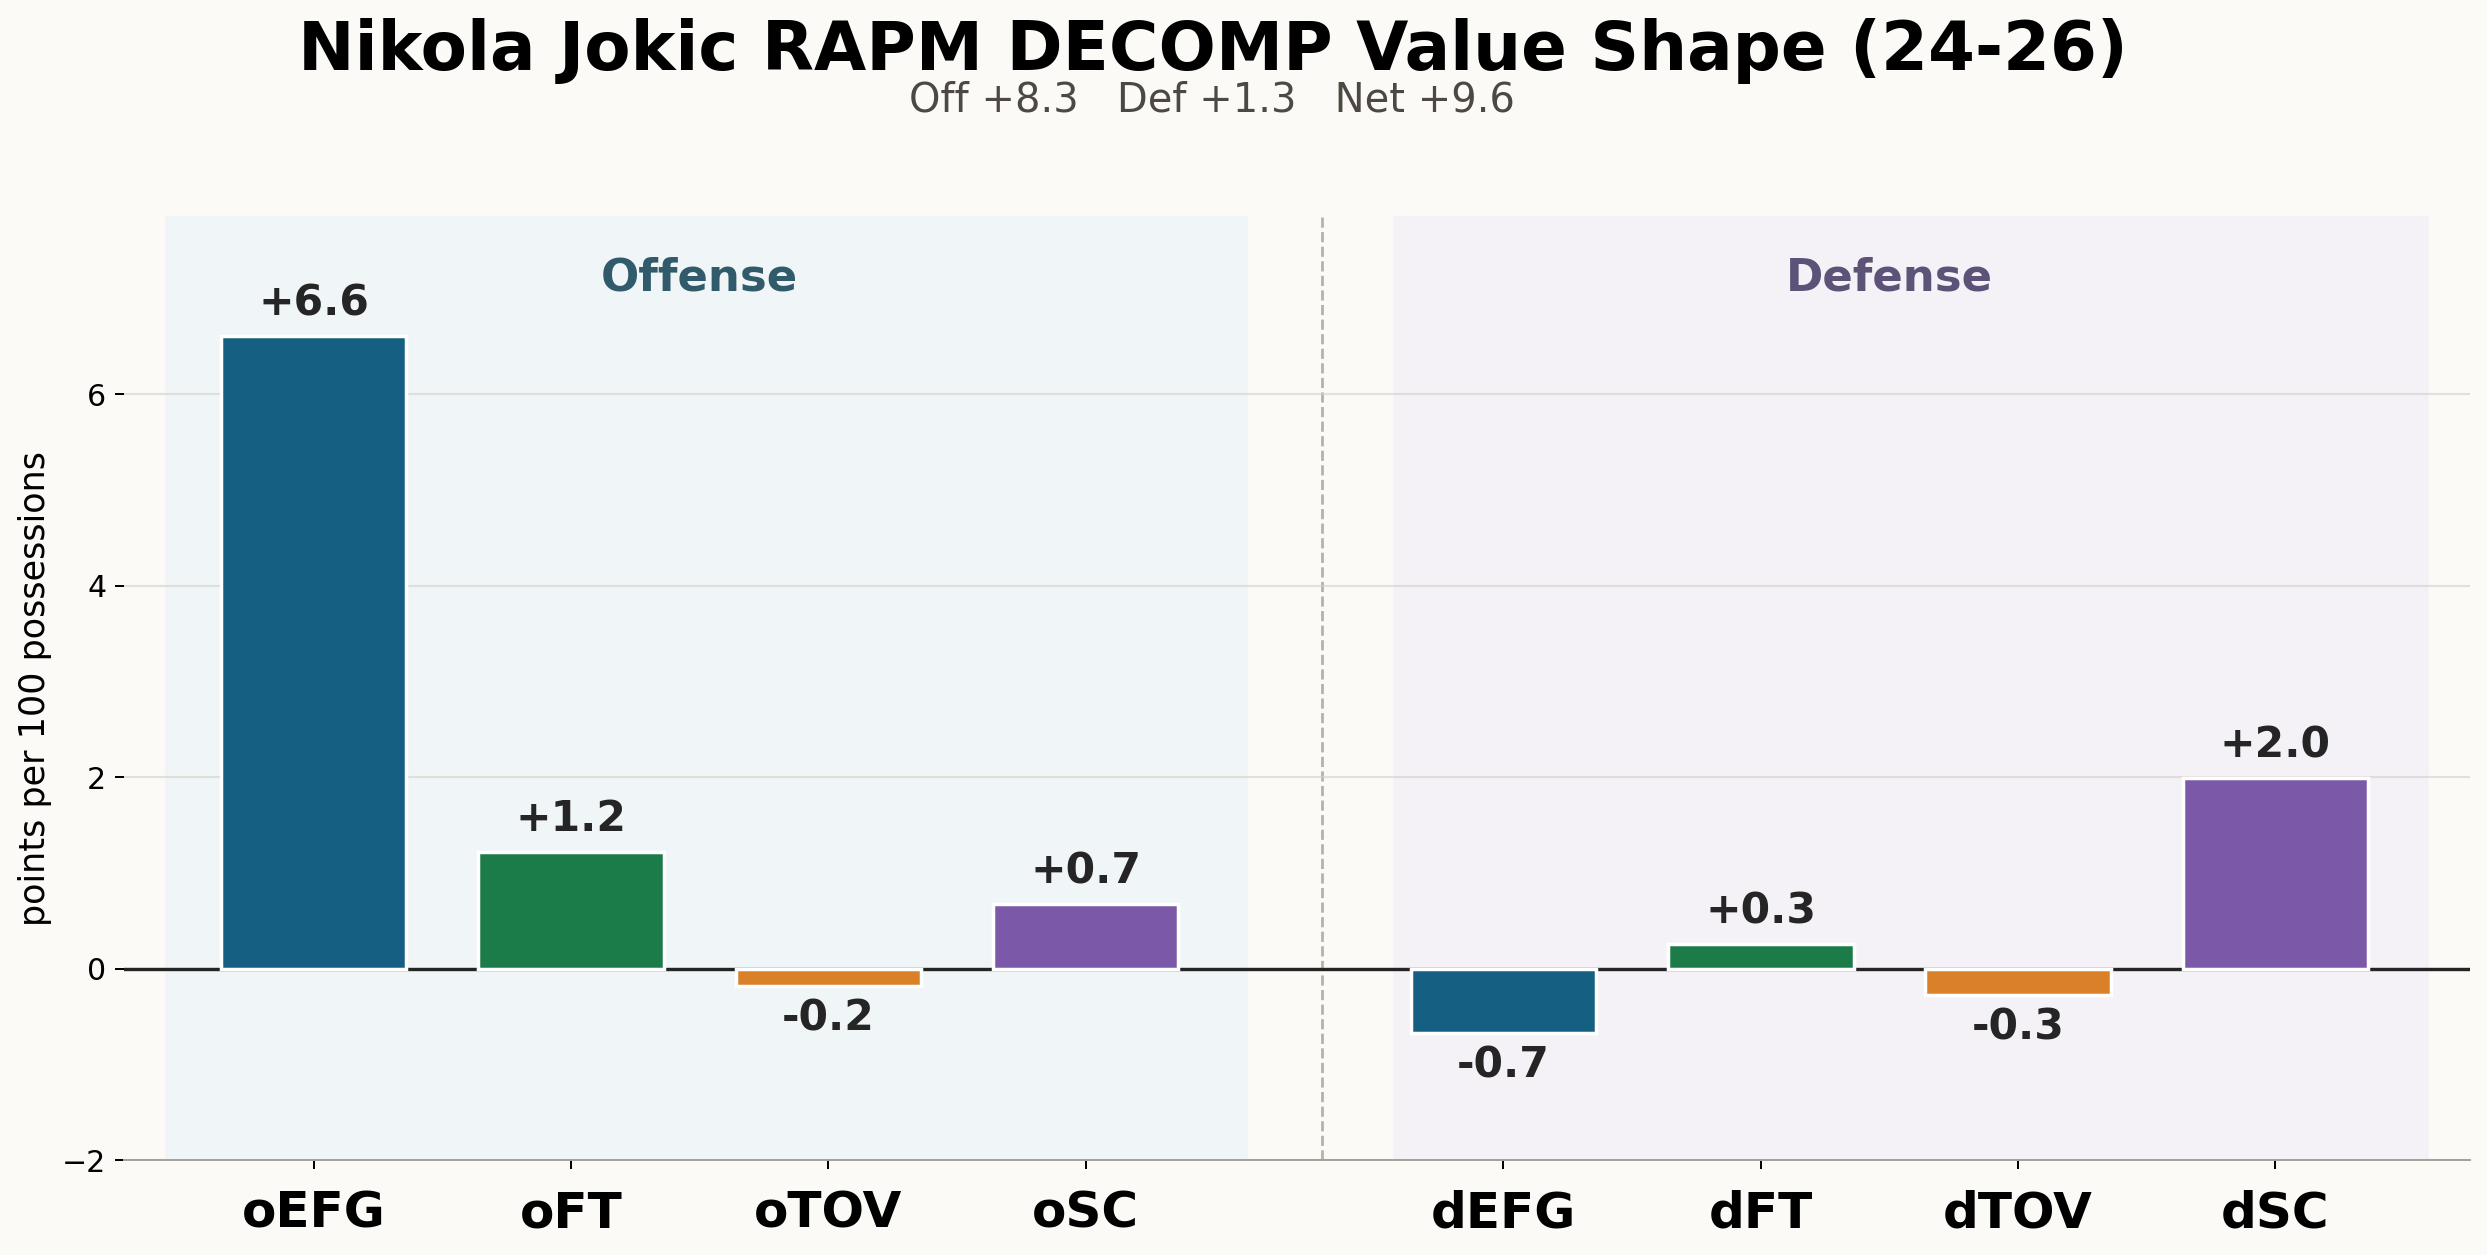
\includegraphics[width=0.92\linewidth]{figures/rapm_decomp_nikola_jokic_value_shape_24_26.png}
\caption{Nikola Jokic's 2024--2026 RAPM DECOMP value shape.  The left side
shows offensive value channels; the right side shows defensive value channels
after sign-flipping so positive means good for the player's team.}
\label{fig:jokic-shape}
\end{figure}

\begin{figure}[h]
\centering
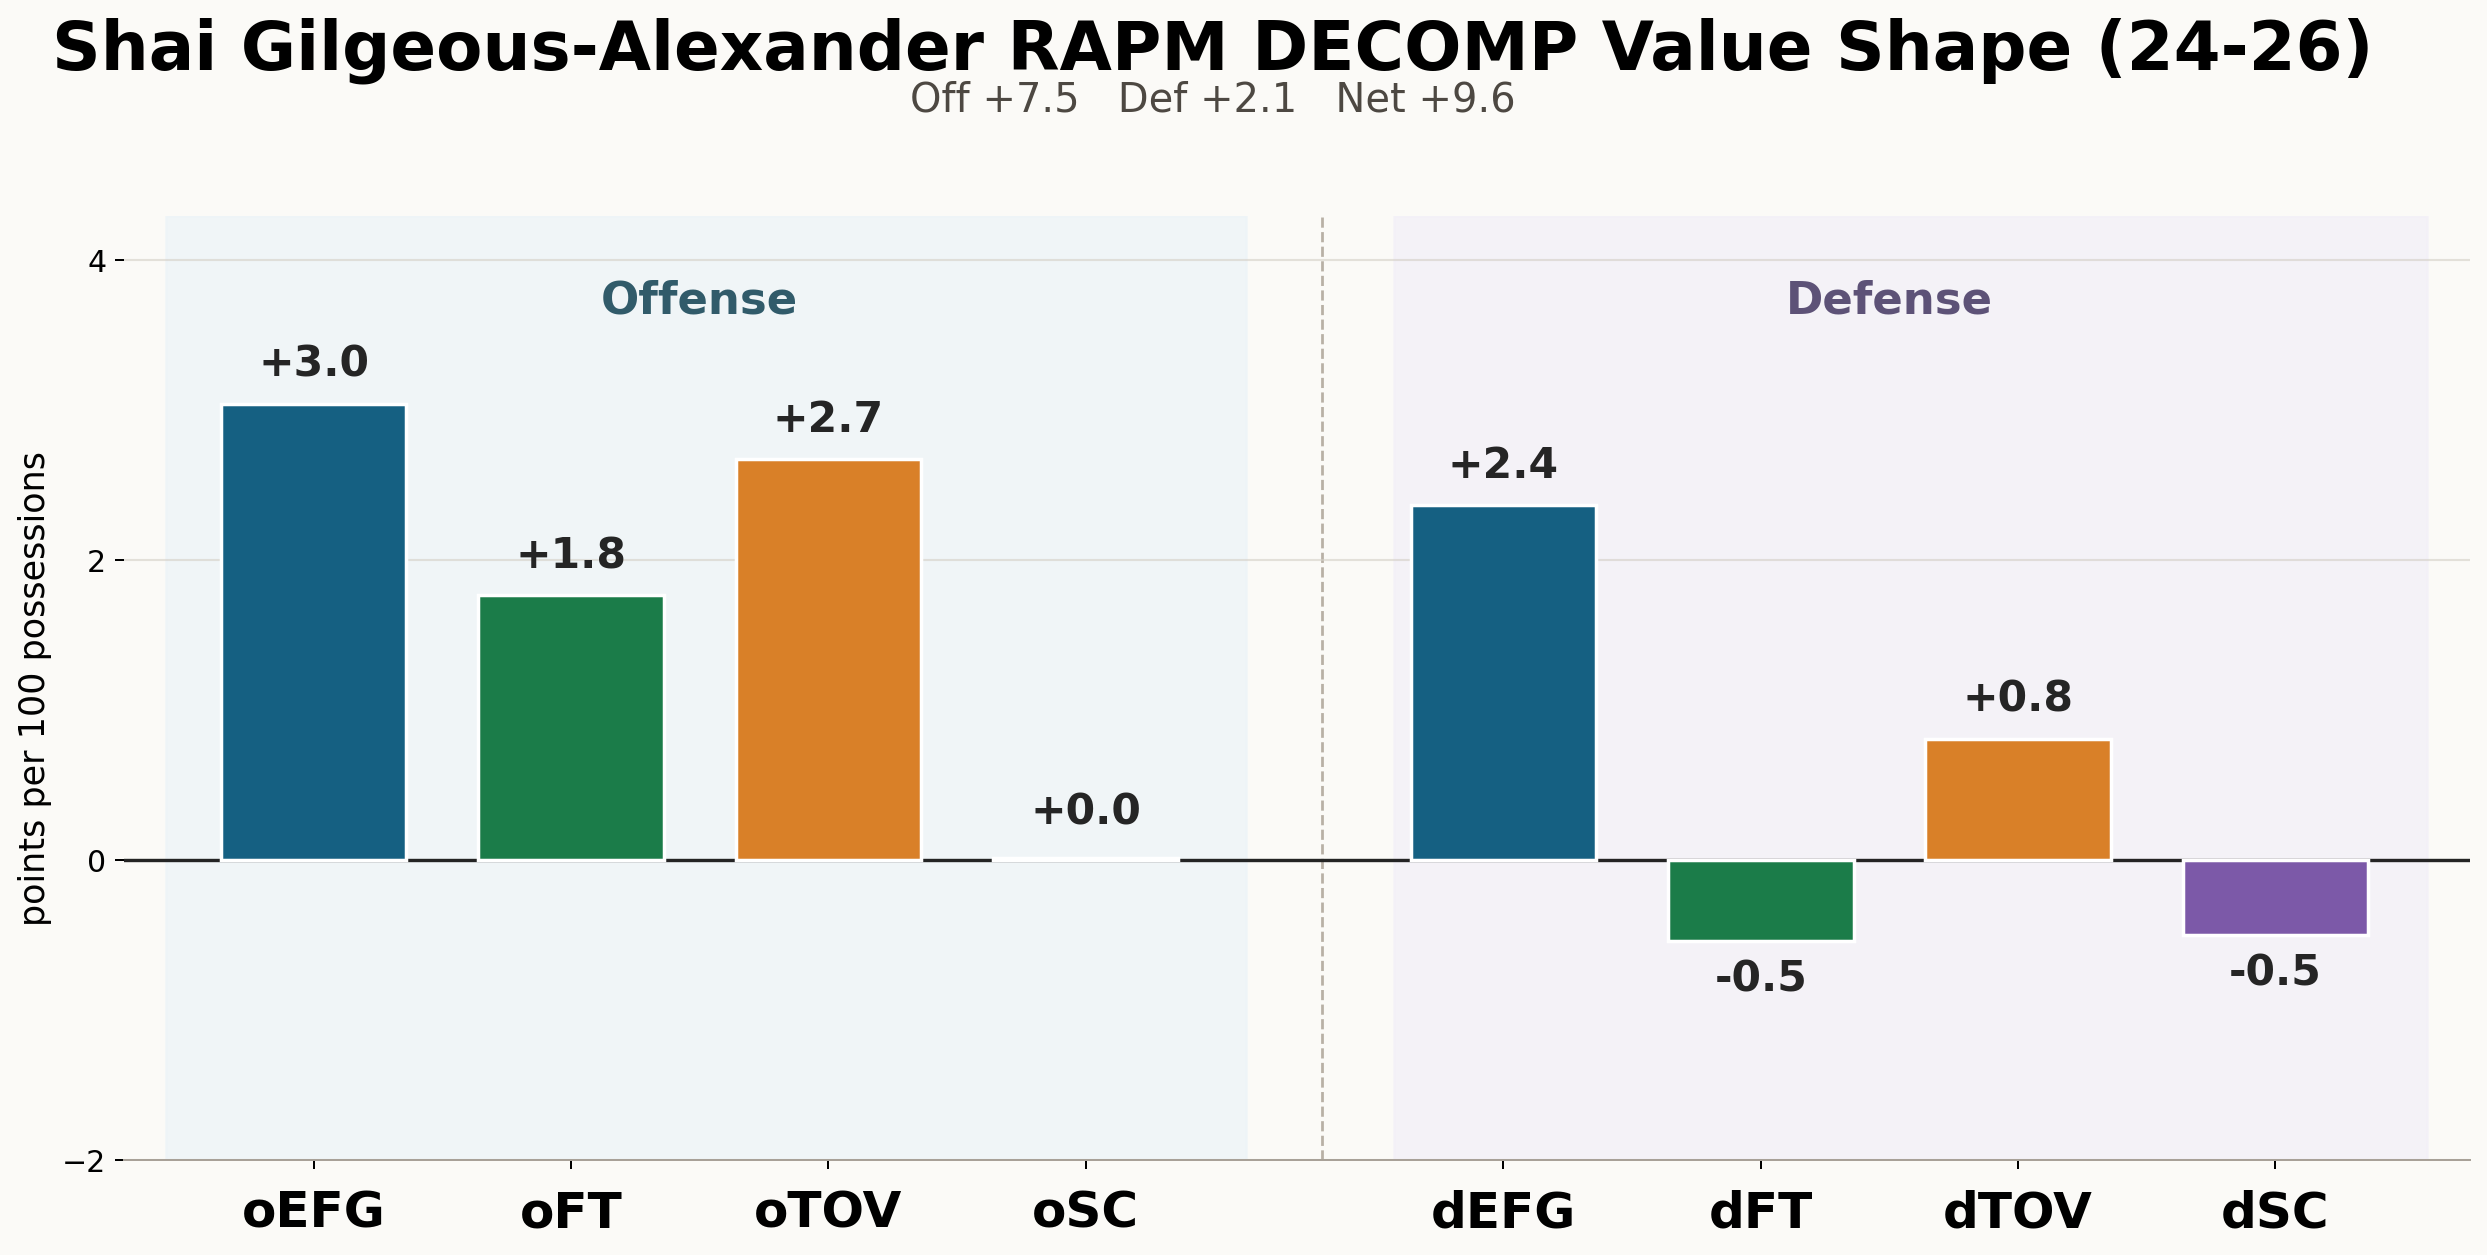
\includegraphics[width=0.92\linewidth]{figures/rapm_decomp_shai_gilgeous_alexander_value_shape_24_26.png}
\caption{Shai Gilgeous-Alexander's 2024--2026 RAPM DECOMP value shape.  The
profile shows a more balanced scoring-and-pressure offensive shape, with a
large first-chance turnover-value term.}
\label{fig:shai-shape}
\end{figure}

\begin{figure}[h]
\centering
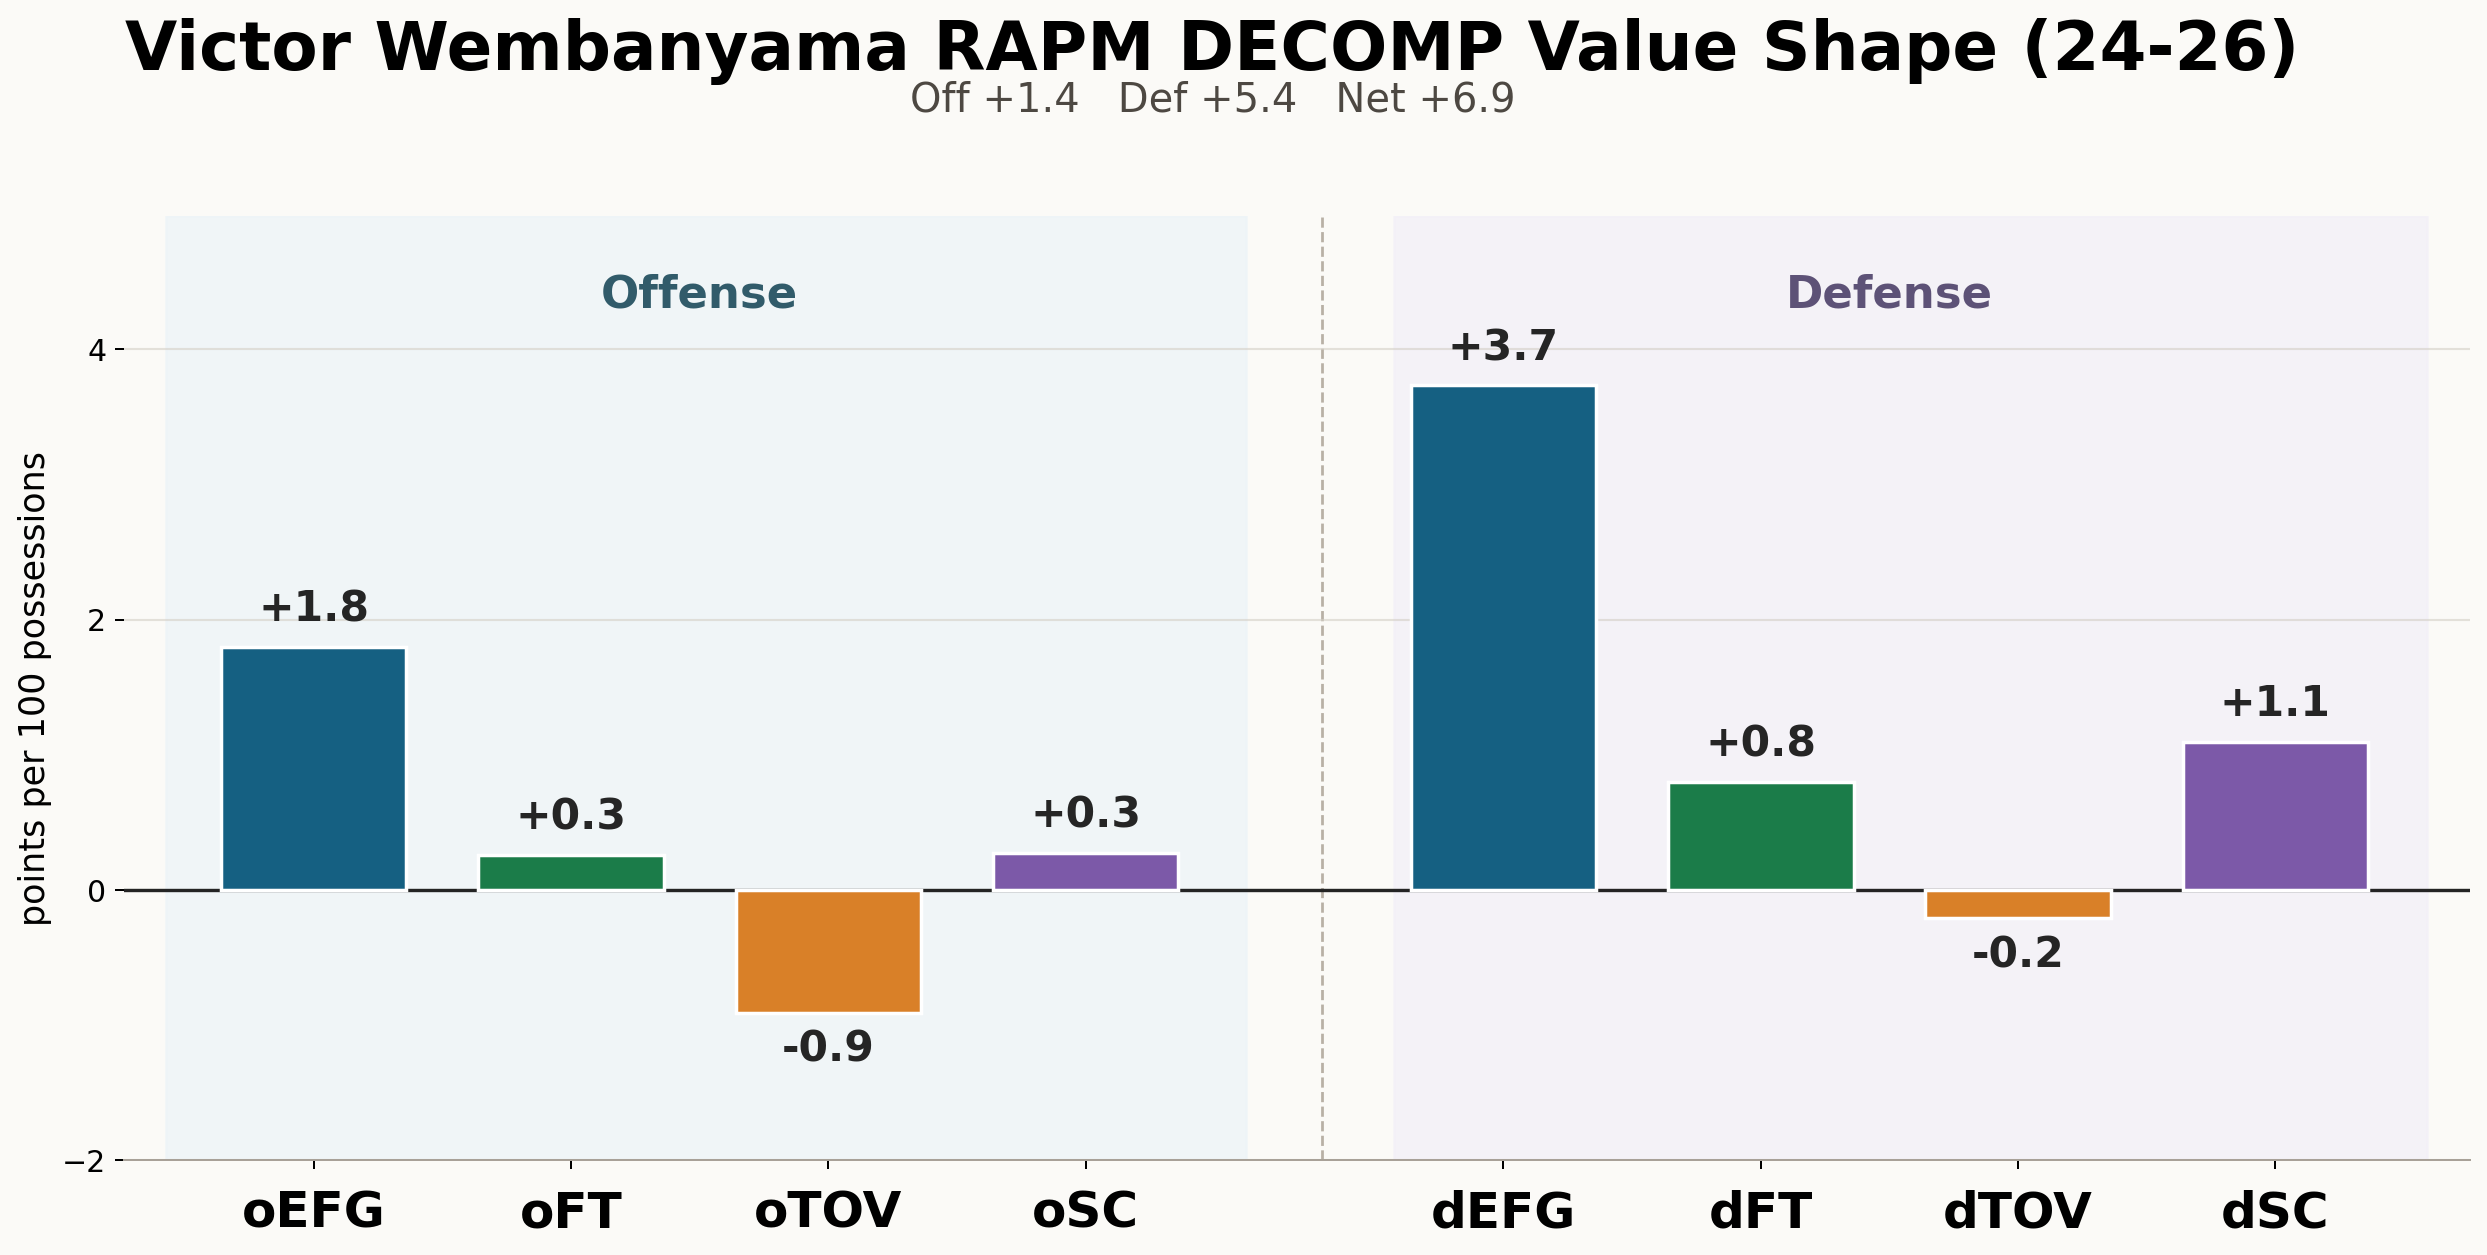
\includegraphics[width=0.92\linewidth]{figures/rapm_decomp_victor_wembanyama_value_shape_24_26.png}
\caption{Victor Wembanyama's 2024--2026 RAPM DECOMP value shape.  The chart
shows a defense-led profile with dominant shot-value prevention and meaningful
offensive first-chance value.}
\label{fig:wembanyama-shape}
\end{figure}

Jokic is an offense-led \texttt{oTS} outlier, with meaningful second-chance
value and a small negative first-chance turnover term.  RAPM DECOMP turns a
one-number offensive coefficient into a recognizable basketball profile: elite
first-chance scoring value, possession extension value, and enough turnover
cost to matter without changing the profile's center of gravity.

Gilgeous-Alexander's offensive profile combines true-shooting value,
free-throw pressure, and a very large positive first-chance turnover-value
term.  His lineups both score efficiently and avoid wasting first-chance
possessions.  That is different from a player whose value is almost entirely
shot making or almost entirely free throws.

Wembanyama is a defensive profile first.  His public shape is dominated by
shot-value prevention, with positive offensive first-chance value and a small
positive second-chance term.  The decomposition says that the large total is not
just a generic defensive coefficient; it is concentrated in suppressing
opponent first-chance scoring value.

\section{Shot-Value Drilldown}

The rolled-up \texttt{oEFG}/\texttt{dEFG} factors are useful because they make
the public table compact.  The atoms underneath them are useful because they
separate location mix from conversion.  Table \ref{tab:shotatoms} shows a small
offensive example.  The columns are not box-score rates.  They are adjusted
point values after lineup controls and public centering.

\begin{table}[h]
\centering
\caption{Example offensive EFG atom profiles, 2024--2026}
\label{tab:shotatoms}
\begin{tabular}{lrrrrrrr}
\toprule
Player & oEFG & RimFreq & RimConv & MidFreq & MidConv & 3Freq & 3Conv\\
\midrule
Nikola Jokic & 3.99 & 0.05 & 0.74 & 0.19 & 0.86 & 0.07 & 0.30\\
Stephen Curry & 3.29 & -0.18 & 0.08 & -0.11 & 0.06 & 0.66 & 0.63\\
Jalen Brunson & 1.60 & -0.18 & 0.02 & 0.63 & 0.30 & -0.06 & 0.19\\
Victor Wembanyama & 1.49 & 0.38 & 0.04 & -0.10 & -0.05 & 0.36 & -0.20\\
\bottomrule
\end{tabular}
\end{table}

The point is not that one atom is the whole explanation.  The point is that one
word, ``shooting,'' can hide very different possession economies.  Curry's
profile loads heavily on three-point value.  Brunson's value has a midrange
shape.  Wembanyama's offensive EFG value comes more from location mix than from
current within-location conversion.  The parent \texttt{oTS} term keeps the
public accounting clean; the atoms make the basketball shape visible.

\section{Factor Correlations}

The factor correlations show that RAPM DECOMP is not merely a leaderboard with
renamed columns.  The channels are related, but not redundant.  In the current
2024--2026 player universe, offensive factors are related but not identical:
\texttt{oEFG} is positively correlated with free-throw value and turnover
value, while second-chance value moves in a different part of the possession
economy.  Defensive factors show their own structure because shot-value
prevention, turnover creation, and second-chance prevention are not the same
skill.

\begin{figure}[h]
\centering
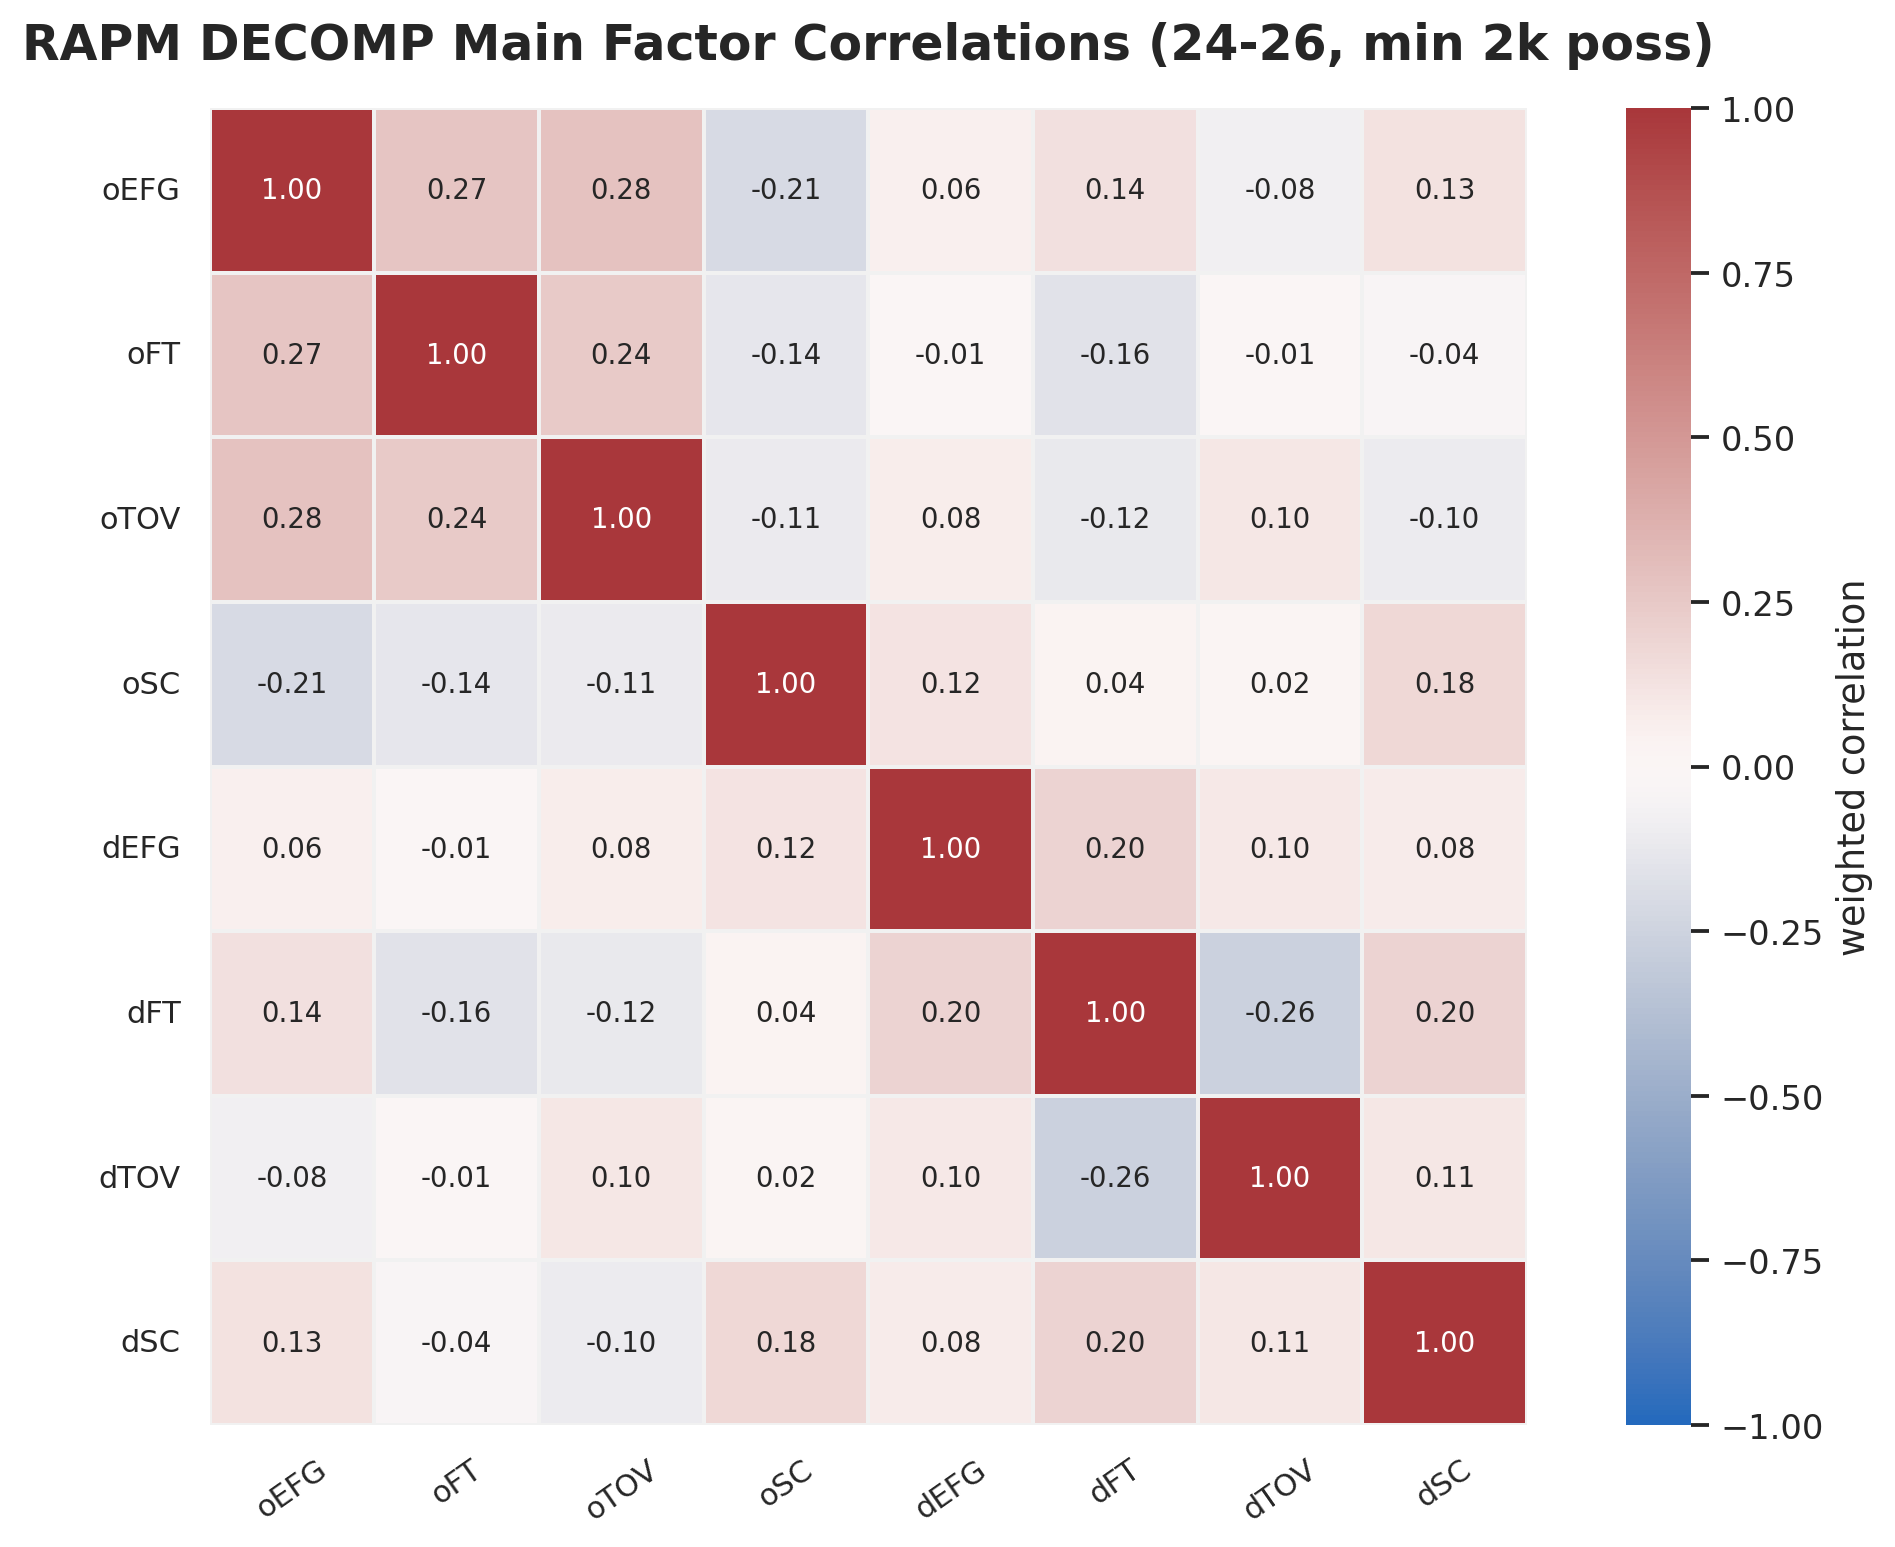
\includegraphics[width=0.92\linewidth]{figures/rapm_decomp_main_factor_corr_24_26.png}
\caption{Possession-weighted correlations among the eight main RAPM DECOMP
factors, 2024--2026 players with at least 2,000 possessions.}
\label{fig:main-corr}
\end{figure}

\begin{figure}[h]
\centering
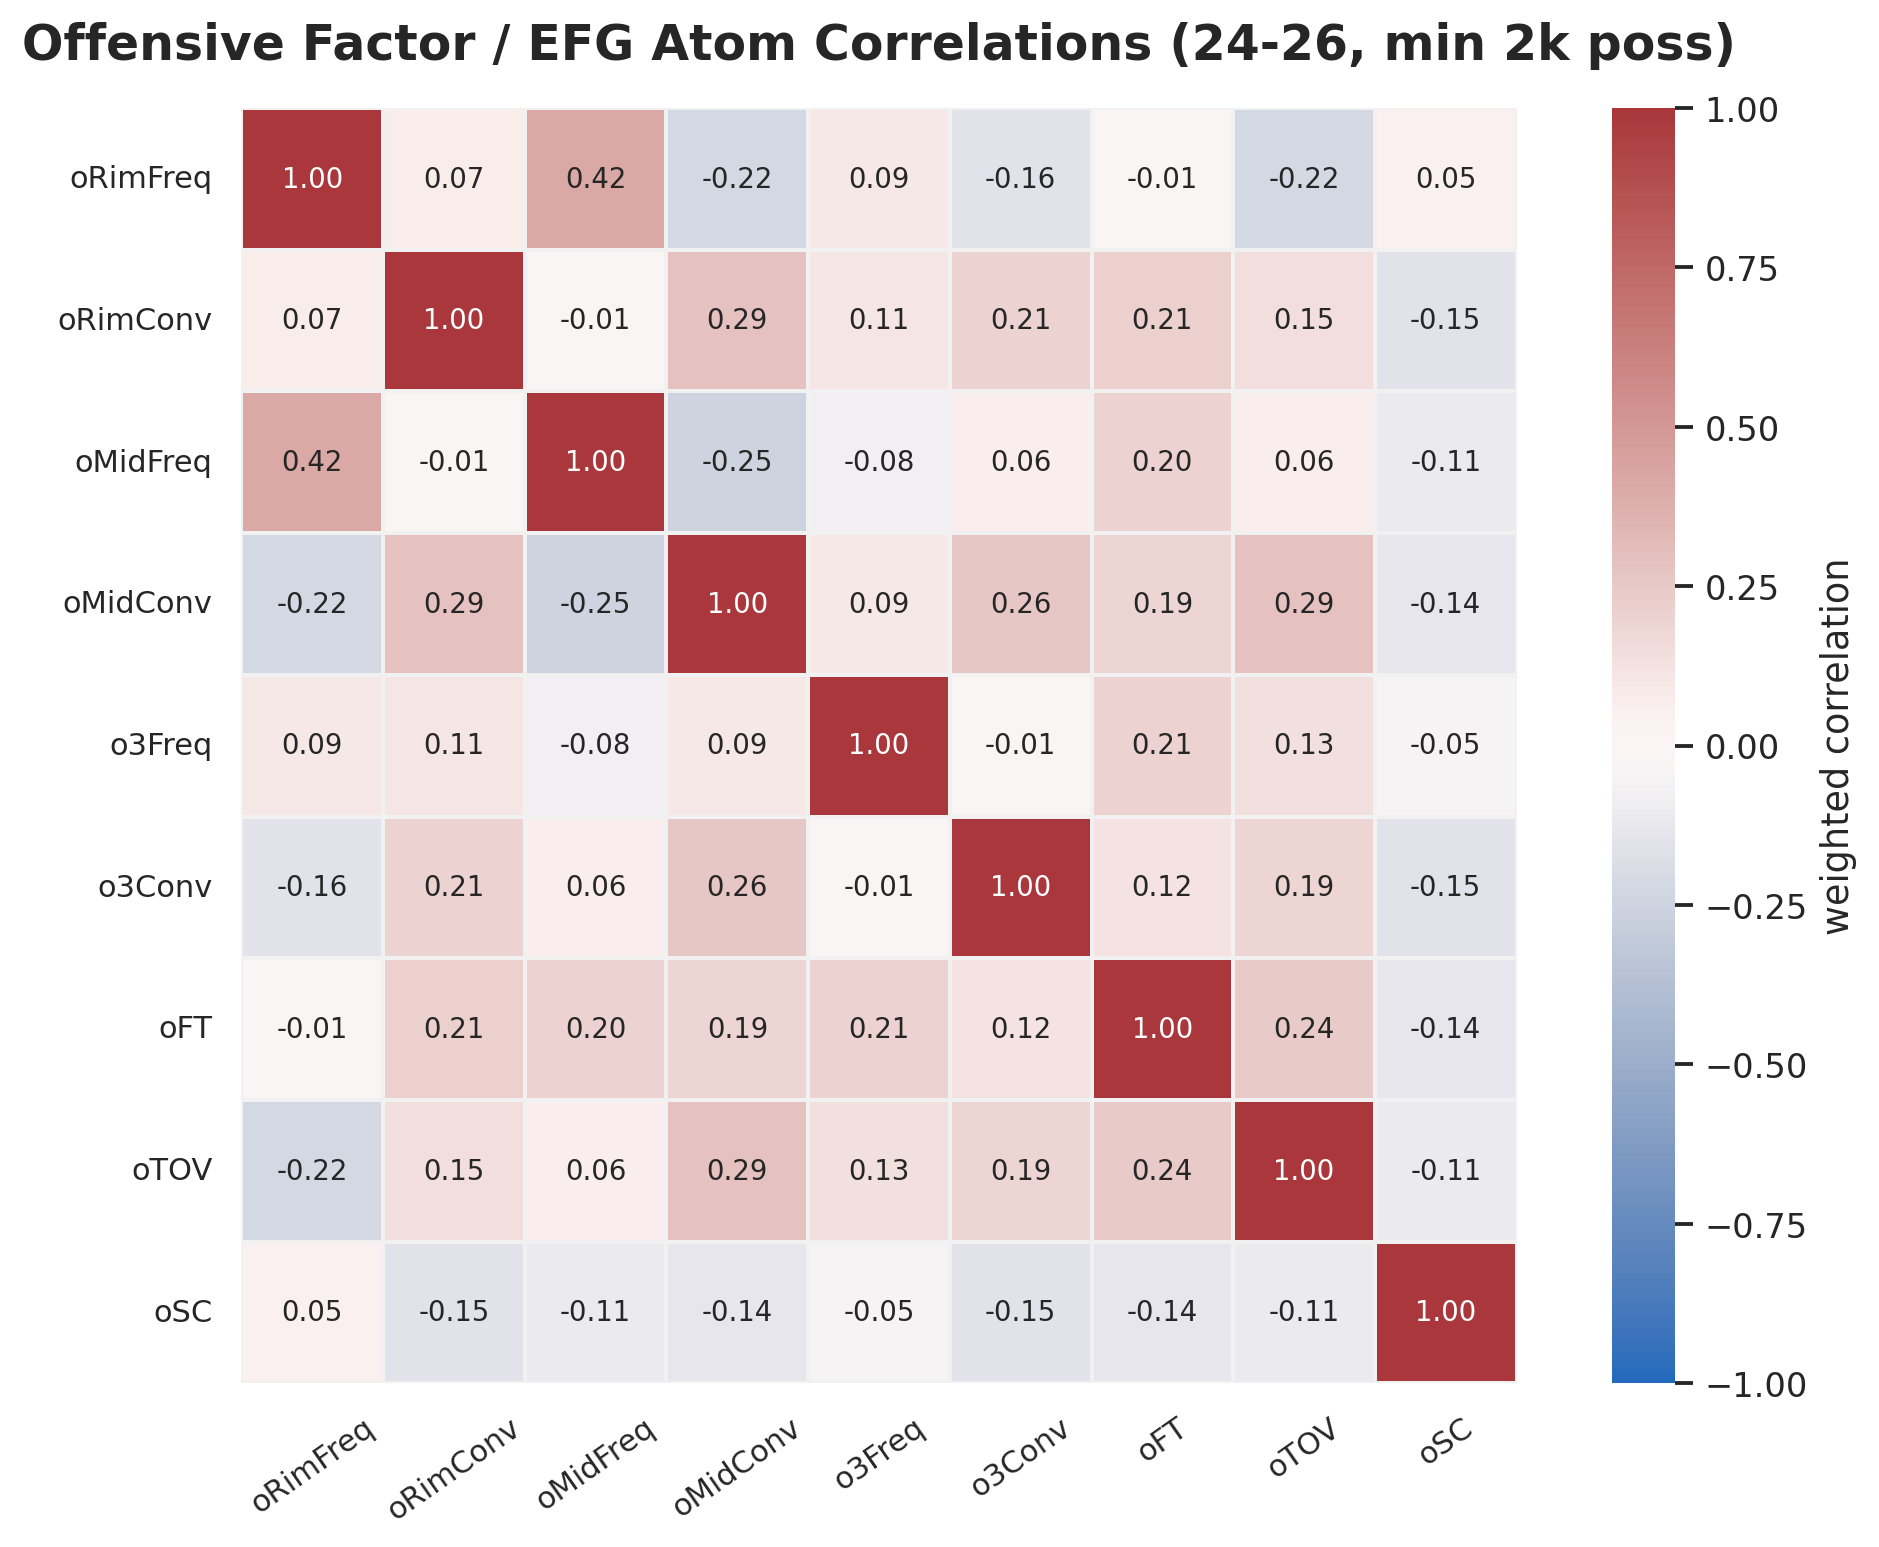
\includegraphics[width=0.88\linewidth]{figures/rapm_decomp_off_factor_corr_24_26.png}
\caption{Possession-weighted offensive factor and EFG-atom correlations,
2024--2026 players with at least 2,000 possessions.}
\label{fig:off-corr}
\end{figure}

\begin{figure}[h]
\centering
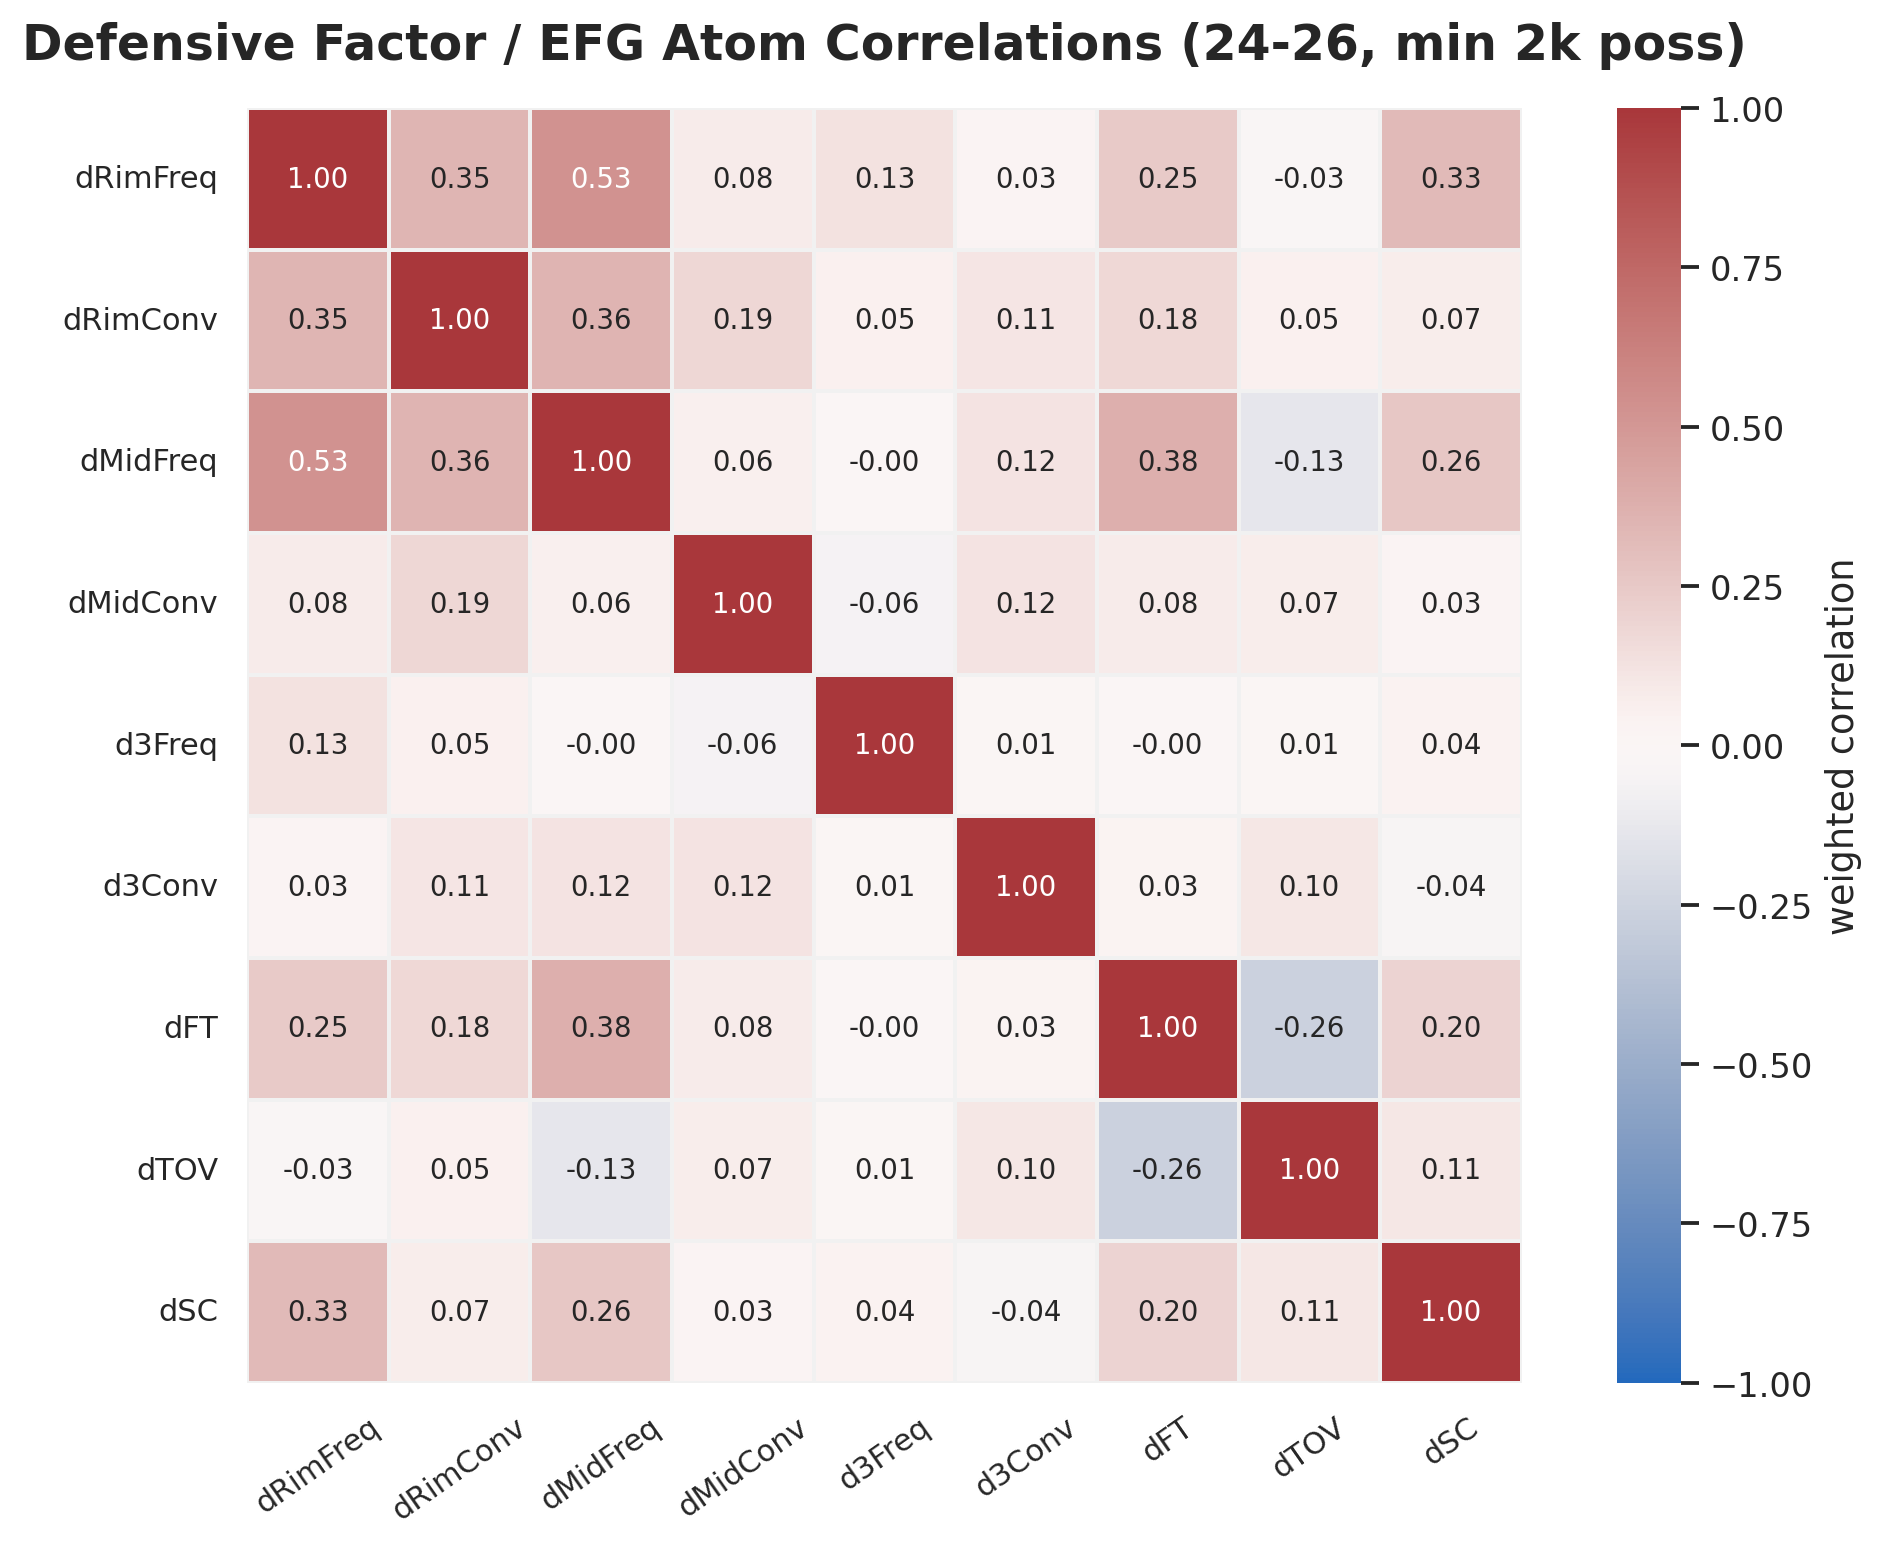
\includegraphics[width=0.88\linewidth]{figures/rapm_decomp_def_factor_corr_24_26.png}
\caption{Possession-weighted defensive factor and EFG-atom correlations,
2024--2026 players with at least 2,000 possessions.}
\label{fig:def-corr}
\end{figure}

\section{Interpretation}

RAPM DECOMP should be read as a map of where adjusted value lands, not as a
complete causal explanation of how the value was generated.  A player can
increase offensive rim value by driving, passing, screening, spacing, or simply
forcing defenses into a particular coverage.  The component says that the
adjusted lineup signal landed in rim value.  It does not say that the player
personally took every valuable rim attempt.

The same caution applies to defense.  Positive defensive shot value means the
opponent's adjusted shot value declined while the player was defending, in the
public good-positive sign convention.  It can include contests, deterrence,
scheme, opponent selection, teammate interaction, and rebounding consequences.
It is a possession-channel estimate, not a film tag.

This limitation is also the source of the metric's usefulness.  RAPM DECOMP
does not replace film or tracking analysis.  It gives them sharper targets.
Instead of asking why a player is good in one number, an analyst can ask why the
player's lineups show high first-chance true-shooting value, negative turnover
value, or unusual second-chance defense.

\section{Historical Coverage}

The long NBA export runs from 1997 through 2026.  That historical reach is
possible because the public decomposition uses possession, scoring,
free-throw, turnover, rebound, lineup, and shot-location information that can
be rebuilt across the long play-by-play archive.  It does not require a
complete tracking-era expected-value model for every season.

Long-window results should still be read carefully.  League shot environments
changed radically between 1997 and 2026.  A midrange frequency value in an
early-2000s context and a midrange frequency value in the current NBA are
measured relative to the loaded run and nuisance-adjusted context, not relative
to a timeless league.  Season effects help, but they do not make eras
identical.

The historical surface is therefore best viewed as evidence of scalability and
as a tool for audited comparison.  It is not a license to ignore era context.
The same arithmetic contract can operate across three decades; specific player
interpretations still require basketball judgment.

\section{Failure Modes and Future Work}

The decomposition can fail in several ways.  First, the target identities can
fail.  If a child target does not add to its parent on the processed rows, then
the public story is false no matter how good the leaderboard looks.

Second, a component can be arithmetically valid but statistically unstable.
Small-sample channels, heavily collinear roles, and low-minute players can move
with ridge penalty, time decay, or window choice.  A component should not be
promoted as stable merely because it is additive.  Split-sample repeatability,
predictive value, ridge sensitivity, time-decay sensitivity, and playoff
sensitivity are the next validation layer.

Third, a component can be semantically too coarse.  Free-throw severity
currently combines trip type and shooter conversion.  That is a valid two-part
split, but it may not answer every foul-drawing question.  The correct response
is to add a new child identity under severity, not to overload the current term.

Fourth, users can overread the columns.  Offensive rim-frequency value is not
the player's own rim-attempt rate.  Defensive three-point conversion value is
not simply opponent luck.  The columns are adjusted possession-channel
estimates.  They are powerful only when interpreted at that level.

The most important future work is uncertainty.  Additivity proves accounting,
not precision.  Public component intervals should be estimated from the final
ridge system or by a resampling design that respects game and lineup structure.
The second priority is a richer shot-quality branch.  Where tracking-era
expected-value data are available, \texttt{oEFG}/\texttt{dEFG} can be split
into pre-shot expected value and making value more directly.  The current
public EFG atoms are deliberately historical and broadly available; they are
not the final form of shot-quality attribution.

\section{Conclusion}

RAPM is valuable because it resists easy box-score stories.  But a single RAPM
coefficient can become its own mystery.  RAPM DECOMP reduces that mystery
without abandoning adjusted plus-minus.  It defines possession-value targets,
solves them through the same lineup-adjusted ridge operator, and publishes the
actual parent coefficient beside factors that add back to the parent.

The claim is intentionally disciplined.  RAPM DECOMP does not solve causality,
replace film, or prove that basketball is simple.  It shows that when a public
impact metric can keep its books, it should.  In the current public exports,
actual RAPM minus the factor sum is only rounding-scale residual.  That gives
analysts a cleaner starting point: not merely who was valuable, but whether the
adjusted value appeared in first-chance scoring, first-chance turnovers,
second-chance value, or defense.

\appendix

\section{Residual Definitions}

For each public player row, \texttt{off} is the actual offensive RAPM
coefficient.  The offensive decomposition residual is:
\[
\text{oRESID}
= \text{off}
- (\text{oEFG}+\text{oFT}+\text{oTOV}+\text{oSC})
= \text{off} - (\text{oFC}+\text{oSC}).
\]
The defensive side uses the public good-positive defensive sign convention:
\[
\text{dRESID}
= \text{def}
- (\text{dEFG}+\text{dFT}+\text{dTOV}+\text{dSC})
= \text{def} - (\text{dFC}+\text{dSC}).
\]
Net residual is:
\[
\text{RESID}
= \text{net\_rapm}
- (\text{off factors}+\text{def factors}).
\]

\section{Public Column Glossary}

\begin{longtable}{p{0.25\linewidth}p{0.65\linewidth}}
\toprule
Term & Meaning\\
\midrule
oFC / dFC & First-chance RAPM: EFG value, free-throw value, and point-valued turnover value before second-chance play.\\
oTS / dTS & First-chance scoring value: EFG value plus free-throw value, interpreted as adjusted first-chance points-per-shot value.\\
oEFG / dEFG & First-chance non-free-throw EFG value, including the baseline shot-value term and location atoms.\\
oFT / dFT & First-chance free-throw value.\\
oTOV / dTOV & Point-valued first-chance scoring opportunity lost or created on true first-chance turnovers.\\
oSC / dSC & Second-chance value after the first offensive miss, with defense sign-flipped so positive is good for the player's team.\\
Rim Frequency & Value of shifting first-chance shots toward or away from rim attempts.\\
Rim Conversion & Within-rim make value after rim frequency is priced.\\
Midrange Frequency & Value of shifting first-chance shots toward or away from midrange attempts.\\
Midrange Conversion & Within-midrange make value after midrange frequency is priced.\\
Three-Point Frequency & Value of shifting first-chance shots toward or away from threes.\\
Three-Point Conversion & Within-three-point make value after three-point frequency is priced.\\
Trip Frequency Value & Average-value first-chance free-throw trip creation.\\
Trip Severity Value & Value above or below the average first-chance trip.\\
\bottomrule
\end{longtable}

\section{Artifact Notes}

The empirical tables in this draft were generated from the local May 2026
pipeline outputs.  The primary public NBA surface is the 2024--2026 all-games
RAPM DECOMP weighted-factor export with score-margin adjustment, season-phase
fixed effects, and side-specific ridge penalties of 2000 and 4000.  The long
historical surface is the 1997--2026 export with the same public schema.  The
six-factor comparison uses the 2021--2026 time-decayed weighted-factor export.

\begin{thebibliography}{9}

\bibitem[Rosenbaum(2004)]{rosenbaum2004}
Dan Rosenbaum.
\newblock Measuring how NBA players help their teams win.
\newblock 82games.com, 2004.

\bibitem[Sill(2010)]{sill2010}
Joseph Sill.
\newblock Improved NBA adjusted plus-minus using regularization and
out-of-sample testing.
\newblock MIT Sloan Sports Analytics Conference, 2010.

\bibitem[Cervone et~al.(2016)]{cervone2016}
Dan Cervone, Alexander D'Amour, Luke Bornn, and Kirk Goldsberry.
\newblock A multiresolution stochastic process model for predicting basketball
possession outcomes.
\newblock \emph{Journal of the American Statistical Association}, 2016.

\end{thebibliography}

\end{document}
